\documentclass[Royal,times,sageh]{sagej}

\usepackage{moreverb,url,natbib, multirow, tabularx}
\usepackage[colorlinks,bookmarksopen,bookmarksnumbered,citecolor=red,urlcolor=red]{hyperref}



% tightlist command for lists without linebreak
\providecommand{\tightlist}{%
  \setlength{\itemsep}{0pt}\setlength{\parskip}{0pt}}



\usepackage{booktabs}
\usepackage{longtable}
\usepackage{array}
\usepackage{multirow}
\usepackage{wrapfig}
\usepackage{float}
\usepackage{colortbl}
\usepackage{pdflscape}
\usepackage{tabu}
\usepackage{threeparttable}
\usepackage{threeparttablex}
\usepackage[normalem]{ulem}
\usepackage{makecell}
\usepackage{xcolor}


\begin{document}


\setcitestyle{aysep={,}}

\title{ActiveCA: Time Use Data from the General Social Survey of Canada
to Study Active Travel}

\runninghead{}

\author{Anon1\affilnum{}, Anon2\affilnum{}, Anon3\affilnum{}}

\affiliation{\affilnum{}{}}



\begin{abstract}
This paper describes \{ActiveCA\}, an open data product with Canadian
time use data. \{ActiveCA\} is an R data package that contains
analysis-ready data related to active travel spanning almost 40 years,
extracted from cycles 2 (1986), 7 (1992), 12 (1998), 19 (2005), 24
(2010), 29 (2015), and 34 (2022) of the Time Use Survey (TUS) cicles
from the General Social Survey (GSS). Active travel is characterized by
mode, with walking being part of every cycle and bicycling starting in
1992. The attributes of active trips are the types of locations of
origins and destinations, the duration of trips, and episode weights for
expanding the trips to population-wide estimates. Based on the year of
the survey, a variety of locations are coded. In earlier cycles, these
include home, work or school, and other's home, whereas in later cycles
these are augmented with locations such as grocery stores, restaurants,
outdoor destinations, and others. The geographical resolution includes
the province and whether the episode was in an urban or rural setting.
\end{abstract}

\keywords{Active; mobility; walking; cycling; travel time; time-use;
General Social Survey}

\maketitle

\section{Introduction}\label{introduction}

The objective of this paper is to introduce \{ActiveCA\}, an open data
product with data from all Time Use Survey (TUS) cycles of the General
Social Surveys (GSSs). Open data products (ODPs) are the outcome of a
process that transforms raw data (open or not) into analysis-ready data,
following a transparent process in which all stages of development
follow open principles \citep{arribas-bel2021}. ODPs, while still open,
differ from general open data in their degree of ease of access, their
heightened usability, and potentially the value they add to the raw
data.

\{ActiveCA\} provides analysis-ready data concerning active travel in
Canada spanning a period of almost 40 years, obtained from the TUS
cycles of the Canadian GSS. The GSS program is designed to provide
cross-sectional data on topics of interest to improve the well-being of
Canadians. As part of this program, every five to seven years the survey
is done on the topic of time use (TUS). Concretely, \{ActiveCA\} covers
Cycles 2 (1986), 7 (1992), 12 (1998), 19 (2005), 24 (2010), 29 (2015),
and 34 (2022) of the TUS. Time use data in these surveys is coded using
a very fine grain, from time spent in chores, leisure, and sleeping, to
time spent working or at school. These surveys have proved valuable in
investigations of mobility and quality of life
\citep{spinneyTransport2009}, the relationship between active travel and
transit use \citep{lachapelleLonger2016}, and travel behavior and time
poverty \citep{kimFacing2024}, to name but a few examples.

Using Public Use Microdata Files (PUMFs) from the Time Use Survey (TUS),
we extracted all data necessary to characterize active travel in Canada
- specifically, episodes in which the activity involved moving between
an origin and a destination by walking or cycling. Although Statistics
Canada provides PUMFs and accompanying documentation for the GSS program
\citep[see][]{statisticscanada2024}, accessing and preparing these files
for analysis is not a straightforward task due to their size and
complexity. The process of extracting information of interest from the
source files is time-consuming, tedious, and challenging and/or prone to
error due to the expertise required to work with these files. To create
\{ActiveCA\} we selected, labelled, and processed the TUS cycles to make
them ready for analysis.

\{ActiveCA\} is distributed as an \texttt{R} package with a number of
data objects and their documentation. \texttt{R} packages contain code,
data, and documentation in a standardized format that can be installed
by R users via a software repository, such as CRAN (Comprehensive R
Archive Network) or GitHub, which makes them an adroit medium to
distribute analysis-ready data.

Given the level of interest in active travel
\citep[e.g.,][]{mccurdySupport2023}, reducing the barriers to using data
contained in rich, but difficult to access and use surveys, such as TUS,
is a worthy endeavour that can only improve data-driven decisions in
transportation, urban, and health policy.

The rest of this paper discusses the sources of data, and the process
implemented to retrieve and package them. Then, we explain how to use
the package and show some selected examples of analysis to whet the
imagination of potential users. This ODP provides not only data that are
easy to use, but also all the code and documentation that make this a
reproducible research project. In summary, \{ActiveCA\} aims to
implement and inspire the best principles of open spatial sciences
\citep{paez_open_2021, brunsdon_opening_2021}.

\section{The Time Use Survey (TUS)
collection}\label{the-time-use-survey-tus-collection}

Statistics Canada \citeyearpar{statisticscanada2024} conducts GSS
surveys to obtain data on social trends to track changes in Canadians'
living conditions and well-being over time. The series of survey on time
use are used to understand how Canadian residents spend and manage their
time, and what factors contribute to their happiness and stress. The GSS
program was created in 1985, and is serialized to provide a collection
of annual, representative cross-sectional surveys.

The topics of the survey cycle every few years to cover topics that
include family, health, social identity, and every five to seven years
time use. The first Canadian TUS done as part of the GSS program was
conducted in 1986, and the most recent was completed in 2022. These Time
Use Surveys \citep{statisticscanada2022} collect data on respondents'
participation and time spent on a wide range of everyday activities
using a 24-hour retrospective diary, with information on the location of
these activities (e.g.~at home, at work, etc.) and, for non-personal
activities, the people who were present with the respondent at the time
of the activity. In addition, time-use surveys also cover topics related
to leisure time, work-life balance, health, commuting, culture and
sports, and many others.

TUS allows researchers to identify the origin and destination of trips,
travel times and modes of transport used, providing a valuable dataset
for analyzing active travel behavior. It also provides the empirical
basis for tools used in transportation analysis, such as the development
of impedance functions for accessibility analysis, a measure of the ease
with which people can reach destinations and opportunities
\citep{hansen1959}. The Canadian TUS is unique at the national level in
collecting detailed information on travel behaviour. Its consistent
application across survey cycles enables the identification of long-term
trends, with some questions present in the questionnaires since the
first application of the survey.

Most respondents to the 2022 TUS completed it online, reflecting
Statistics Canada's effort to adapt to technological changes and growing
time demands by offering greater flexibility and convenience
\citep{statisticscanada2022}. While such methodological changes may
affect data comparability over time, it is not possible to determine
whether observed differences result from actual population changes or
shifts in data collection methods. Despite rigorous efforts to ensure
data quality, the use of electronic questionnaires may have influenced
estimates. Statistics Canada assessed the impact of collection mode on a
limited set of key questions, constrained by sample size. Importantly,
none of the variables used in this research are \texttt{R} package in
the 2022 PUMF User Guide as unsuitable for trend analysis.

Until 2022, Statistics Canada employed a telephone-based sampling frame,
which was replaced by a dwelling-based frame in the most recent cycle.
Each survey cycle spans a 12-month period, typically from July to the
following July. The target population includes all Canadians aged 15 and
over, excluding residents of the Yukon, Northwest Territories, and
Nunavut, full-time institutional residents, and individuals living on
Indigenous reserves.

The survey encompasses both rural and urban areas, including
metropolitan and non-metropolitan regions, to ensure a diverse and
representative sample. For sampling, the ten provinces were divided into
geographic strata. Several Census Metropolitan Areas (CMAs) - such as
St.~John's, Halifax, Saint John, Montreal, Quebec City, Toronto, Ottawa,
Hamilton, Winnipeg, Regina, Saskatoon, Calgary, Edmonton, and Vancouver
- were treated as separate strata. Additional strata grouped other CMAs
within Quebec, Ontario, and British Columbia, as well as non-CMA areas
within each province.

The Public Use Microdata are released by Statistics Canada in two files:
a \emph{Main file} and an \emph{Episode file}. The files are linked by
keys that identify households, individuals, and episodes (i.e.,
activities) conducted by individuals. We discuss these files in more
detail in the following section.

\subsection{The Main file}\label{the-main-file}

The \emph{Main file} of the time use survey compiles a large array of
aggregated data, summarizing the answers to the questionnaire that
describe households and individuals, as well as derived variables that
summarize the respondents' use of time use across different activities,
locations, and social interactions. This file documents the time and
duration that respondents allocate to each activity and location. The
\emph{Main file} provides a overview of daily routines and social
dynamics, not focusing on individual activity episodes. Additionally,
this file categorizes activities into bigger groups and subcategories,
facilitating the data's analytical utility with additional metrics such
as total transit time, time spent with household members, and counts of
activities and episodes.

Table \ref{tab:main-2015-unprocessed} shows the first ten rows and first
six variables of the TUS PUMF 2015 \emph{Main file} (Cycle 29). Each row
in the table correspond to a survey respondent, while the columns refer
the following information: record identification (\texttt{PUMFID}), the
person's weight (\texttt{WGHT\_PER}), the month the survey data was
collected (\texttt{SURVMNTH}), the respondent's age group
(\texttt{AGEGR10}), the respondent's sex (\texttt{SEX}), and the
respondent's marital status (\texttt{MARSTAT}).

The \emph{Main file} of the 2015 GSS surveys includes a total of 17,390
respondents, representing 29,766,399 individuals and 848 variables. For
discrete variables, Statistics Canada has assigned specific codes to the
possible values, with each code accompanied by a label. For instance, in
the case of the variable \texttt{SURVMNTH}, a value of \texttt{1} means
\texttt{January\ 2016}, \texttt{2} means \texttt{February\ 2016},
\texttt{3} corresponds to \texttt{March\ 2016}, and so on.

As shown in Table \ref{tab:main-2015-unprocessed}, the variables are not
labeled. Additionally, the format of the tables (comma-separated values)
does not allow for the specification of variable types (whether a
variable is continuous or discrete), which can lead to mistakes analysts
who have limited experience working with PUMFs.

\begingroup\fontsize{8}{10}\selectfont

\begin{ThreePartTable}
\begin{TableNotes}
\item \textit{Note: } 
\item Legend: PUMFID: record identification. WGHT\_PER:  person weight. SURVMNTH: survey month of data collection. AGEGR10: age group of the respondent. SEX: sex of the respondent. MARSTAT: marital status of the respondent.
\end{TableNotes}
\begin{longtable}[t]{cccccc}
\caption{\label{tab:gss-main-file-2015}\label{tab:main-2015-unprocessed}Visualization of the first ten lines and first six columns of the Main file of the 2015 GSS.}\\
\toprule
PUMFID & WGHT\_PER & SURVMNTH & AGEGR10 & SEX & MARSTAT\\
\midrule
10000 & 616.6740 & 7 & 5 & 1 & 5\\
10001 & 8516.6140 & 7 & 5 & 1 & 1\\
10002 & 371.7520 & 1 & 4 & 2 & 1\\
10003 & 1019.3135 & 3 & 6 & 2 & 5\\
10004 & 1916.0708 & 9 & 2 & 1 & 6\\
\addlinespace
10005 & 1952.2015 & 4 & 1 & 1 & 6\\
10006 & 5761.5528 & 8 & 1 & 1 & 6\\
10007 & 466.0426 & 6 & 5 & 2 & 3\\
10008 & 2479.2991 & 2 & 2 & 2 & 1\\
10009 & 1436.1641 & 8 & 6 & 1 & 3\\
\bottomrule
\insertTableNotes
\end{longtable}
\end{ThreePartTable}
\endgroup{}

\subsection{The Episode file}\label{the-episode-file}

The episode is a much bigger file that records detailed data for each
activity episode reported by respondents. Each episode represents a
single activity and its duration, and the sum of all episodes throughout
the day adds up to 24 hours. Each entry in this file includes the start
and end times of the activity, the duration, location, and accompanying
social context, informing when and where activities occurred and with
whom. The focus of the \emph{Episode file} is not on the characteristics
of the respondents, but on the characteristics of the activities, and
the data are structured around the numerous activity instances that
compose a day of the respondent. Although respondent-specific
characteristics are not included within the \emph{Episode file}, it is
possible to link the \emph{Main file} and the \emph{Episode file} by
using a key present in both the \emph{Main} and \emph{Episode files}.

Similar to Table \ref{tab:main-2015-unprocessed}, which displayed an
example of the \emph{Main file} structure, Table
\ref{tab:ep-2015-unprocessed} presents the first seven episodes for the
record identification number 10041 and some variables from the TUS PUMF
2015 \emph{Episode file} (Cycle 29). Each row in the table corresponds
to an episode associated with the specified record identification
(\texttt{PUMFID} = \texttt{10041}), including the episode's weight
(\texttt{WGHT\_EPI}), episode number (\texttt{EPINO}), activity code
(\texttt{TUI\_01}), episode duration (\texttt{DURATION}), and episode
location (\texttt{LOCATION}).

In total, the \emph{Episode file} of the 2015 GSS surveys contains
274,108 records, representing 461,837,622 episodes and 527 variables
detailing the episodes. Similar to the \emph{Main file}, Statistics
Canada has created codes for the discrete variables, with each value
corresponding to a label.

In the case illustrated in Table \ref{tab:ep-2015-unprocessed}, this
respondent began the diary description by sleeping at home
(\texttt{TUI\_01\ =\ 1} and \texttt{LOCATION\ =\ 300}) for 210 minutes,
followed by 40 minutes of personal hygiene (\texttt{TUI\_01\ =\ 2}). The
respondent then spent 15 minutes on personal care activities, such as
getting ready for school, supervising homework, reading, playing,
reprimanding, or providing educational or emotional support, as
indicated by \texttt{TUI\_01\ =\ 27.} Next, they recorded a travel
episode, walking for 15 minutes (\texttt{TUI\_01\ =\ 7} and
\texttt{LOCATION\ =\ 315}), where both the origin and destination were
their home. Such trips, where the journey starts and finishes at home,
can be classified as recreational or leisure trips. Next, the respondent
spent 3 hours searching for a job (\texttt{TUI\_01\ =\ 9}), took a
15-minute lunch break (\texttt{TUI\_01\ =\ 6}), and then cleaned the
house (\texttt{TUI\_01\ =\ 18}) for two hours. Table
\ref{tab:ep-2015-unprocessed} displays only six variables out of the 527
available. As shown, since the dataset does not label the variable
values, decoding them can be both time-consuming and challenging.

\begingroup\fontsize{8}{10}\selectfont

\begin{ThreePartTable}
\begin{TableNotes}
\item \textit{Note: } 
\item Legend: PUMFID: record identification. EPINO: episode number. WGHT\_EPI: episode's weight. TUI\_01: activity code. DURATION: episode's duration. LOCATION: episode's location.
\end{TableNotes}
\begin{longtable}[t]{cccccc}
\caption{\label{tab:gss-epi-file-2015}\label{tab:ep-2015-unprocessed}Visualization of the seven first episodes of the record number 10041.}\\
\toprule
PUMFID & EPINO & WGHT\_EPI & TUI\_01 & DURATION & LOCATION\\
\midrule
10041 & 1 & 1353.818 & 1 & 210 & 300\\
10041 & 2 & 1353.818 & 2 & 40 & 300\\
10041 & 3 & 1353.818 & 27 & 15 & 300\\
10041 & 4 & 1353.818 & 7 & 15 & 315\\
10041 & 5 & 1353.818 & 9 & 180 & 300\\
\addlinespace
10041 & 6 & 1353.818 & 6 & 15 & 300\\
10041 & 7 & 1353.818 & 18 & 120 & 300\\
\bottomrule
\insertTableNotes
\end{longtable}
\end{ThreePartTable}
\endgroup{}

\section{Data process}\label{data-process}

Figure \ref{fig:process-figure} presents a diagram illustrating the
processes applied to the \emph{Main} and \emph{Episode files} to create
the \{ActiveCA\} datasets. For each TUS cycle, we reviewed the
\emph{Episode files} to identify movement episodes involving walking or
cycling. This allowed us to also select the activities immediately
before and after the movement episode, helping to infer the trip's
purpose and determine its origin and destination. Active trips were
identified by their corresponding activity codes, accounting for
variations across survey cycles.

Next, we labeled the coded variables with their appropriate
descriptions, classifying each origin and destination, mode of travel,
and time spent in the active trip. Categorical variables were converted
into factor variables, and ordinal variables were defined as ordered
factors.

For the \emph{Main files}, we selected socioeconomic variables to help
profile individuals engaged in active travel episodes. These included
key indicators such as age group, sex, marital status, and number of
children, among others. As with the \emph{Episode files}, we labeled and
factored the coded variables. Using the appropriate identifiers, we
joined the Episode and \emph{Main files} to determine the province and
the type of population centre - whether it is a CMA, a Census
Agglomeration (CA), or a non-CMA/CA area.

As output, the \{ActiveCA\} package provides processed datasets of
walking and cycling episodes by year, a unified dataset that contains
all walking and cycling episodes across TUS cycles, and processed main
files (not unified, as socioeconomic and demographic variables and their
categories differ across TUS cycles).

\begin{figure}

{\centering 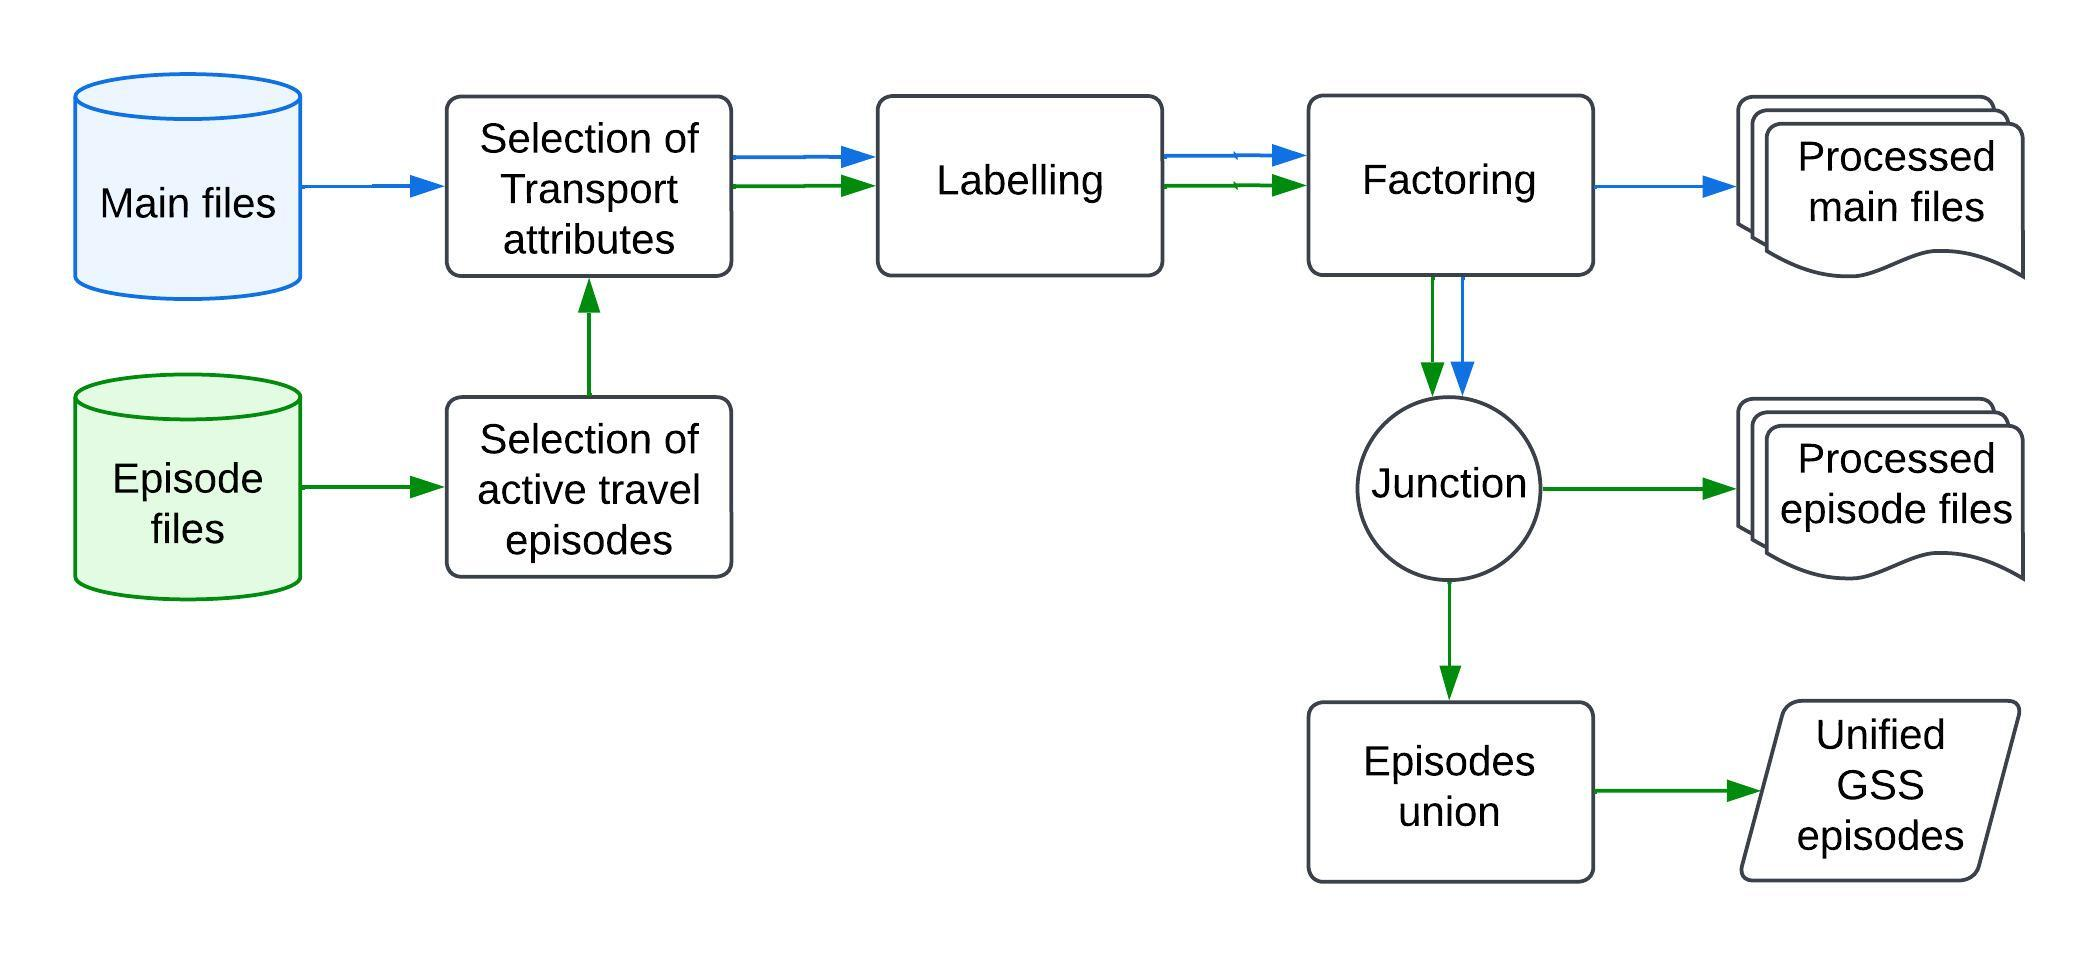
\includegraphics[width=1\linewidth]{Manuscript-figures/RPackages - ActiveCA} 

}

\caption{Diagram with the processes applied to the main (blue arrows) and episode files (green arrows) to obtain the ActiveCA datasets.}\label{fig:process-figure}
\end{figure}

\section{\{ActiveCA\} data sets}\label{activeca-data-sets}

This section presents some potential applications of the \{ActiveCA\}
\texttt{R} package. In fact, we expect that the application of this
package to extend beyond our pre-imagined range of uses. The
installation instruction and also some examples of application of the
\{ActiveCA\} \texttt{R} package are available in the \texttt{vignettes},
available in the Github repository.

\subsection{Active episodes}\label{active-episodes}

Table \ref{tab:processed-obs} displays the total number of records
processed for Main and \emph{Episode files}. For the \emph{Main files},
a total of 101,667 records were processed, referring to all records from
the Time Use Surveys from 1986 to 2022, that together represents more of
181,526,641 respondents. It also presents the total cases of active
trips episodes identified. In total 23,513 records with register of
active travel activity. Together, these records account for 44,316,110
episodes.

\begingroup\fontsize{8}{10}\selectfont

\begin{longtable}[t]{rr>{}r|rr}
\caption{\label{tab:table_df_processed}\label{tab:processed-obs}Total number and weighted sum of records processed.}\\
\toprule
\multicolumn{1}{c}{ } & \multicolumn{2}{c}{Main} & \multicolumn{2}{c}{Episode} \\
\cmidrule(l{3pt}r{3pt}){2-3} \cmidrule(l{3pt}r{3pt}){4-5}
Year & Count & Weighted & Count\_ep & Weighted\_ep\\
\midrule
2022 & 12336 & 32136802 & 1765 & 6041032\\
2015 & 17390 & 29766399 & 3496 & 6634387\\
2010 & 15390 & 28075610 & 4615 & 8516753\\
2005 & 19597 & 26095819 & 5866 & 7583838\\
1998 & 10749 & 24260137 & 1789 & 3606987\\
\addlinespace
1992 & 9815 & 21294313 & 1635 & 3691918\\
1986 & 16390 & 19897562 & 4347 & 8241196\\
\bottomrule
\end{longtable}
\endgroup{}

Table \ref{tab:main-2015-processed} shows the first ten rows and first
six variables of the TUS PUMF 2015 Main File (Cycle 29), displayed in
\ref{tab:main-2015-unprocessed} before our processing. Table
\ref{tab:ep-2015-processed} presents the walking episodes for the record
identification number \texttt{10041} from the TUS PUMF 2015
\emph{Episode file} (Cycle 29), previously displayed in Table
\ref{tab:ep-2015-unprocessed}. Only the unique active travel episode
appear in Table \ref{tab:ep-2015-processed} since the records were
filtered to select cases with walking or cycling episodes. For both
cases, Tables \ref{tab:main-2015-processed} and
\ref{tab:ep-2015-processed} contain labeled variables, facilitating the
interpretation of the data.

\begingroup\fontsize{8}{10}\selectfont

\begin{ThreePartTable}
\begin{TableNotes}
\item \textit{Note: } 
\item Legend: PUMFID: record identification. WGHT\_PER:  person weight. SURVMNTH: survey month of data collection. AGEGR10: age group of the respondent. SEX: sex of the respondent. MARSTAT: marital status of the respondent.
\end{TableNotes}
\begin{longtable}[t]{cccccc}
\caption{\label{tab:gss-processed-file-2015}\label{tab:main-2015-processed}Visualization of the first ten lines and first six columns of the 2015 TUS Main File.}\\
\toprule
PUMFID & WGHT\_PER & SURVMNTH & AGEGR10 & SEX & MARSTAT\\
\midrule
10000 & 616.6740 & July & 55 to 64 years & Male & Divorced\\
10001 & 8516.6140 & July & 55 to 64 years & Male & Married\\
10002 & 371.7520 & January & 45 to 54 years & Female & Married\\
10003 & 1019.3135 & March & 65 to 74 years & Female & Divorced\\
10004 & 1916.0708 & September & 25 to 34 years & Male & Single, never married\\
\addlinespace
10005 & 1952.2015 & April & 15 to 24 years & Male & Single, never married\\
10006 & 5761.5528 & August & 15 to 24 years & Male & Single, never married\\
10007 & 466.0426 & June & 55 to 64 years & Female & Widowed\\
10008 & 2479.2991 & February & 25 to 34 years & Female & Married\\
10009 & 1436.1641 & August & 65 to 74 years & Male & Widowed\\
\bottomrule
\insertTableNotes
\end{longtable}
\end{ThreePartTable}
\endgroup{}

\begingroup\fontsize{8}{10}\selectfont

\begin{ThreePartTable}
\begin{TableNotes}
\item \textit{Note: } 
\item Legend: PUMFID: record identification. EPINO: episode number. WGHT\_EPI: episode's weight. TUI\_01: activity code. DURATION: episode's duration. LOCATION: episode's location.
\end{TableNotes}
\begin{longtable}[t]{rrlrlll}
\caption{\label{tab:gss-processed-file-2015}\label{tab:ep-2015-processed}Visualization of the active travel episode for the record number 10041 of the 2015 GSS survey.}\\
\toprule
PUMFID & WGHT\_EPI & Activity & Duration & Origin & Destination & Mode\\
\midrule
10041 & 1353.818 & Transport to or from activity & 15 & Home & Home & Walking\\
\bottomrule
\insertTableNotes
\end{longtable}
\end{ThreePartTable}
\endgroup{}

\subsection{Descriptive statistics}\label{descriptive-statistics}

Considering all TUS analyzed, we identified 23,513 episodes that
recorded active travel episodes, with trip duration ranging from 0 to
900 minutes, to twelve different destinations. \{ActiveCA\} includes all
these episodes ready for analysis. Table \ref{tab:table-01} presents
descriptive statistics on walking and cycling trips between 1986 and
2022, with measures of trip duration in minutes. The 1986 survey did not
include bicycle trips.

\begingroup\fontsize{8}{10}\selectfont

\begin{longtable}[t]{>{}llccccccc}
\caption{\label{tab:table-01}\label{tab:table-01}Descriptive statistics for episodes with active transport records}\\
\toprule
\multicolumn{2}{c}{ } & \multicolumn{7}{c}{Year} \\
\cmidrule(l{3pt}r{3pt}){3-9}
Mode & Statistic & 1986 & 1992 & 1998 & 2005 & 2010 & 2015 & 2022\\
\midrule
 & Maximum & 660 & 300 & 255 & 515 & 480 & 900 & 480\\
\nopagebreak
 & Mean & 21 & 21 & 12 & 12 & 13 & 18 & 19\\
\nopagebreak
 & Median & 15 & 10 & 5 & 10 & 10 & 10 & 15\\
\nopagebreak
 & Minimum & 1 & 1 & 1 & 0 & 0 & 5 & 5\\
\nopagebreak
\multirow[t]{-5}{*}{\raggedright\arraybackslash \textbf{Walking}} & Standard deviation & 31 & 25 & 17 & 16 & 17 & 27 & 24\\
\cmidrule{1-9}\pagebreak[0]
 & Maximum &  & 240 & 90 & 180 & 153 & 120 & 150\\
\nopagebreak
 & Mean &  & 28 & 24 & 20 & 19 & 25 & 40\\
\nopagebreak
 & Median &  & 15 & 15 & 15 & 10 & 20 & 30\\
\nopagebreak
 & Minimum &  & 5 & 2 & 1 & 1 & 5 & 5\\
\nopagebreak
\multirow[t]{-5}{*}{\raggedright\arraybackslash \textbf{Cycling}} & Standard deviation &  & 36 & 18 & 18 & 23 & 20 & 20\\
\bottomrule
\end{longtable}
\endgroup{}

Table \ref{tab:table-01} shows that, until 2022 the median values for
walking trips were 10 minutes, increasing to 15 minutes in the last
survey. In the case of cycling trips, the duration fluctuated over the
years, ranging from 10 to 30 minutes. The table also highlights very
high maximum values, particularly for walking trips, with recorded
episodes exceeding 4 hours in all cases.

\{ActiveCA\} also enables visual analysis of active travel in Canada
using exploratory data analysis techniques. Figure \ref{fig:figure-01}
shows walking trips from 2022 through heat maps. This graph uses color
gradients to represent the percentage of trips between various origins
and destinations, with darker colors indicating higher percentages and
lighter colors representing less frequent routes. For conciseness, we
omitted the heat maps for the other years analyzed.

In 2022, \texttt{home} served as a central hub for most trips, with
fewer than 10\% of journeys not involving it as either a starting point
or destination. The most common trip types were from \texttt{home} to
\texttt{work\ or\ school} (17\%) and the reverse, from
\texttt{work\ or\ school} to \texttt{home} (13\%). Notably, 7\% of trips
began and ended at \texttt{home}, often reflecting leisure activities
such as short walks or dog walking. \texttt{Grocery\ stores} were also a
key destination, comprising 10\% of trips departing from \texttt{home.}

\begin{figure}

{\centering 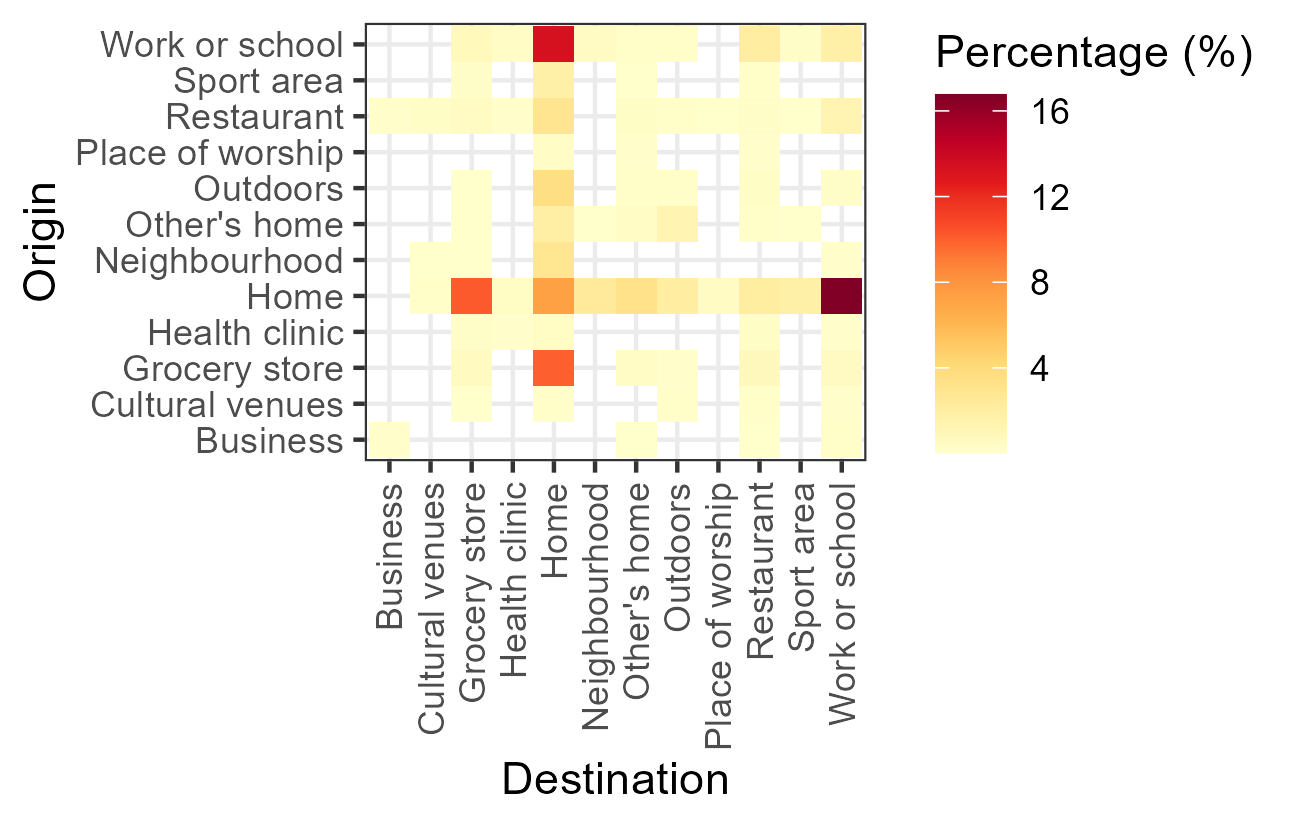
\includegraphics[width=1\linewidth]{Manuscript-figures/walking_hm_2022} 

}

\caption{Percentage of walking trips categorized by origin and destination}\label{fig:figure-01}
\end{figure}

The \{ActiveCA\} dataset also includes information on the type of
population centre in which respondents reside - specifically, whether
they live in a CMA, a CA, or outside these areas - as well as the
respondent's province. This information is important, as patterns of
active travel often differ between metropolitan and non-metropolitan
populations. For example, Table \ref{tab:cma-durations} presents the
median walking durations by population centre type and province for
2022. Overall, respondents living in CMA/CA areas tend to report higher
median walking durations compared to those living outside these centres.
The most pronounced difference is observed in Nova Scotia: metropolitan
residents reported a median walking duration of 30 minutes, whereas
non-metropolitan residents reported a median of only 5 minutes.

\begin{table}
\centering
\caption{\label{tab:cma-durations}\label{tab:cma-durations}Differences in walking duration between provinces and population centre type.}
\centering
\resizebox{\ifdim\width>\linewidth\linewidth\else\width\fi}{!}{
\fontsize{8}{10}\selectfont
\begin{threeparttable}
\begin{tabular}[t]{lrr}
\toprule
\multicolumn{1}{c}{ } & \multicolumn{2}{c}{Population centre type} \\
\cmidrule(l{3pt}r{3pt}){2-3}
Province & CMA/CA & non CMA/CA\\
\midrule
Alberta & 15 & 5\\
British Columbia & 15 & 10\\
Manitoba & 10 & 10\\
New Brunswick & 5 & 5\\
Newfoundland and Labroador & 20 & 10\\
\addlinespace
Nova Scotia & 30 & 5\\
Ontario & 15 & 15\\
Prince Edward Island &  & 5\\
Quebec & 15 & 15\\
Saskatchewan & 10 & 5\\
\bottomrule
\end{tabular}
\begin{tablenotes}
\item \textit{Note: } 
\item CMA denotes Census Metropolitan Area and CA denotes Census agglomeration.
\end{tablenotes}
\end{threeparttable}}
\end{table}

The package also enables obtaining insights from the main processed
files. Figure \ref{fig:figure-stress} present how the level of stress
varied among respondents depending on their marital status in 2022.
According to this plot, married respondents reported the highest level
of stress, relating to feel stressed every day, with 15\% of possible
cases.

\begin{figure}

{\centering 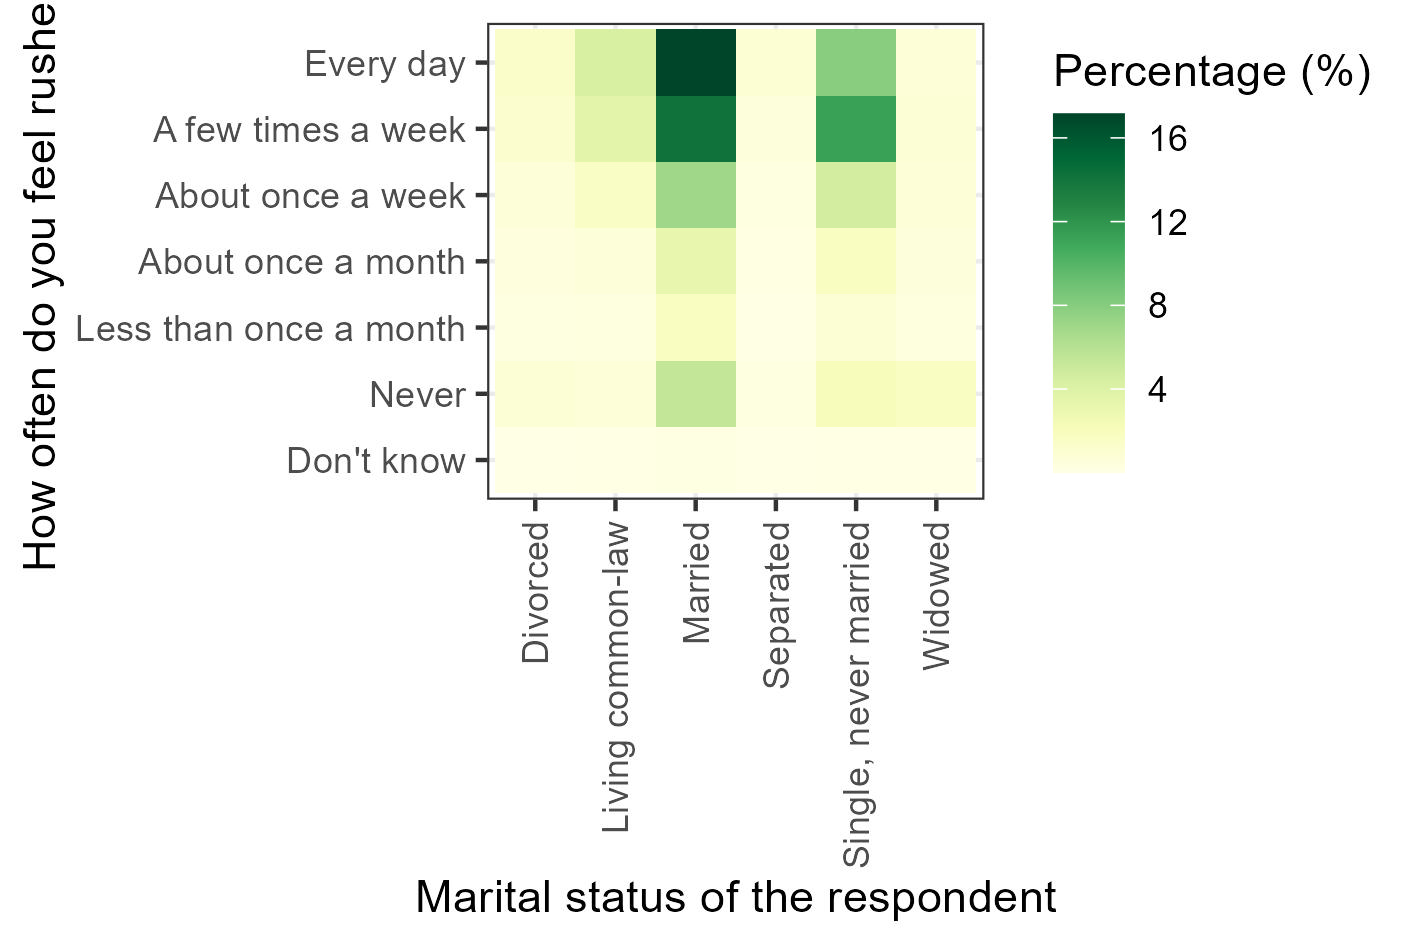
\includegraphics[width=1\linewidth]{Manuscript-figures/main_stress_figure} 

}

\caption{Level of stress among respondents of different marital statuses (2015).}\label{fig:figure-stress}
\end{figure}

\section{Python integration}\label{python-integration}

\{ActiveCA\} also provides a Jupyter Notebook containing a
\texttt{Python} script that demonstrates how to read \texttt{R} data
files (.rda) and convert them into Pandas DataFrames. This process
allows users to work with and utilize the datasets available in
\{ActiveCA\} within a \texttt{Python} project.

\section{Concluding remarks}\label{concluding-remarks}

This paper presents \{ActiveCA\}, an open data product that provides
analysis-ready data from Cycles 2 (1986), 7 (1992), 12 (1998), 19
(2005), 24 (2010), 29 (2015), and 34 (2022) of TUS GSSs on active travel
in Canada. In the form of an \texttt{R} data package, \{ActiveCA\} was
developed after collecting, cleaning, and processing the survey data,
providing information on origins, destinations, and duration of active
travel, as well other information.

Although we did not select non-AT episodes, the process for obtaining
them is very similar to that used for selecting AT episodes. Researchers
interested in non-AT modes can use our framework to guide their
methodology, making the small but necessary adjustments. We focused
exclusively on AT episodes because the \{ActiveCA\} package is part of a
larger project aimed at analyzing the historical evolution of active
travel behaviour in Canada.

The value of \{ActiveCA\} lies in its transparency, accessibility, and
ease of use, which facilitates the addition of complementary data sets
in the future. R users can seamlessly explore TUS walking and cycling
episodes, with the option to suggest enhancements to the package as
needed. This article adopts the structure proposed by Anastasia and Páez
\citeyearpar{soukhov2023}, whose work provided essential guidance for
the creation of this package. Similarly, we aim to contribute to the
academic community by promoting transparent research practices that
encourage replication and innovation in related fields. We believe that
\{ActiveCA\} will serve as a basis for further research on TUS and for
the integration of additional data by the authors or the wider open
source community.

\section{Declaration of Conflicting
Interests}\label{declaration-of-conflicting-interests}

The author(s) declared no potential conflicts of interest with respect
to the research, authorship, and/or publication of this article.

\section{Funding}\label{funding}

The author(s) disclosed receipt of the following financial support for
the research, authorship, and/or publication of this article: This work
was supported by the Social Sciences and Humanities Research Council of
Canada (\emph{More description about the funding source after the review
process}).

\section{ORCID}\label{orcid}

Author 1

Author 2

Author 3

\section{Data availability statement}\label{data-availability-statement}

The \{ActiveCA\} R data package can be found and installed on Github
(\emph{link}).

For review purposes, the package is currently available as a tar.gz file
that can be installed by R. The file can be obtained from this anonymous
location:

\url{https://user.fm/files/v2-3d261d0b2aa47fcad096cd9e49fd5cf8/ActiveCA.zip}

\bibliographystyle{sageh}
\bibliography{bibfile.bib}


\end{document}
